\chapter{Diskretisierung}

Partielle Differentialgleichungen (PDGn) n-ter Ordnung für skalares $u(x)$ sind von der Form
\begin{equation}
  F(x, t, u(x), Du(x), \dots, D^nu(x))=0, \qquad x\in\Omega\subset\mathbb{R}^d \; .
\end{equation}
Sie unterliegen Randbedingungen (für die Zeitvariable auch Anfangsbedingung genannt), die je nach Problemstellung auf Teilen des Randes formuliert sind. Beispielsweise ist die Auslenkung einer eingespannten Membran am Ortsrand fest, während in der Zeit lediglich für $t_0$ ein Randwert vorliegt (am linksseitigen Rand der Zeitdomäne).

Die LvNG \eqref{eq:lvn} ist eine lineare PDG zweiter Ordnung in $d=2$ Dimensionen. Sie ist weder elliptisch, noch parabloisch, noch hyperbolisch\footnote{Dies ist ersichtlich anhand der Eigenwerte der Koeffizientenmatrix zweiter Ableitungen $T=\text{diag}(0,1,-1)$ für Gleichung \eqref{eq:lvn_first}}.
Ferner bildet $u\in C^2(\Omega)$ in den Raum der komplexen Zahlen ab. Damit unterscheidet sich das Problem bereits grundlegend von den zumeist in der Literatur vorkommenden Problemstellungen. Die stationäre LvNG hingegen ist hyperbolisch. In diesem Kapitel soll ein Verfahren entwickelt werden, welches bislang noch nicht zur Anwendung gekommen ist im Kontext der LvNG: das \emph{Discontinuous-Galerkin}\index{Discontinuous-Galerkin Verfahren} (DG) Verfahren. Die Ausführungen orientieren sich an dem praxisnahen Buch von Hesthaven und Warburton \cite{buch}.

Zunächst wird ein Überblick über verschiedene, gängige numerische Verfahren gegeben. Vor- und Nachteile werden skizziert, wenngleich die Numerik partieller Differentialgleichungen ein großes Forschungsgebiet ist und somit die verschiedenen angedeuteten Probleme sich möglicherweise nur in einer oberflächlichen Betrachtung als solche äußern.

\section{Übersicht}
Bei der Diskretisierung einer PDG sind zwei grundlegende Fragestellungen zu berücksichten:
\begin{enumerate}
  \item Auf welche Weise wird die Lösung $u(x,t)$ durch eine diskrete Lösung $u_h(x,t)$ genähert?
  \item Wie ist die Verbindung zwischen diskretisierter Lösung und zugrundeliegender PDG?
\end{enumerate}
Als Folge einer unterschiedliche Beantwortung dieser Fragen wurden zahlreiche Verfahren entwickelt, die jeweils spezifische Vor- und Nachteile aufweisen. Im Folgenden werden in knapper Form drei Verfahren vorgestellt und  gegeneinander verglichen. In dieser Reihenfolge nimmt die Komplexität zu, denn die Schwächen des einen Verfahrens führen jeweils zu der nächst allgemeineren Formulierung.

\subsection{Finite Differenzen}\index{Finite Differenzen}\label{sec:FD}
Die partiellen Ableitungen werden bei diesem Verfahren durch eine endliche (finite) Anzahl von Differenzen genähert. Zur Formulierung der n-ten Ableitung einer Funktion $f(x)$ im Punkt $x_0$ wird die zugehörige Taylorreihe bis zur n-ten Ordnung verwendet. Der Punkt $x_0$ entstammt einem Gitter, welches das Gebiet $\Omega$ diskretisiert. Dieser Ansatz setzt inhärent voraus, dass eine Funktion sich hinreichend genau durch ein lokales Polynom niedriger Ordnung nähern lässt. Damit ist zeitgleich Frage (1) beantwortet.

Die Antwort auf die zweite Frage bestimmt dann die Koeffizienten der lokalen Polynome. Durch Einsetzen der Näherung $u_h(x,t)$ in die PDG folgt ein Residuum
\begin{equation}
  \mathcal{R}(x,t)\equiv F(x,t, u_h(x), Du_h(x), \dots, D^nu_h(x,t)) \; ,
\end{equation}
welches i.A. nicht verschwindet, denn sonst wäre ${u_h(x,t) = u(x,t)}$ die exakte Lösung. Zur Bestimmung der Koeffizienten (Freiheitsgrade) wird daher beispielsweise gefordert, dass auf den Gitterpunkten ${\mathcal{R}(x^k,t)=0}$ verschwindet.

Das Verfahren ist besonders leicht zu implementieren. Es ist robust, effizient und wird von einer umfangreichen Literatur gestützt. Für zeitabhängige Probleme folgt aus der Ortsdiskretisierung eine explizite semidiskrete Form, was eine Flexibilität in der Wahl der Zeitschritt-Methode ermöglicht. In höherdimensionalen Problemen $d>1$ erfordert das Verfahren jedoch eine Tensorprodukt-Struktur der Basisfunktionen, sodass letztlich komplexe Geometrien $\Omega\subset{\mathbb{R}^d}$ nicht gut abgebildet werden können. Ferner führen Unstetigkeiten in den Randbedingungen oder internen Schichten (wie zum Beispiel der Potentialsprung in Abbildung \ref{fig:pot1}) zu Problemen aufgrund der simplen, zugrundeliegenden Diskretisierung.

\subsection{Finite Volumen}\index{Finite Volumen}
Für erhöhte geometrische Flexibilität und insbesondere für nichtlineare Erhaltungsgleichungen eignet sich das Finitive Volumen (FV) Verfahren. Das Gebiet $\Omega$ wird dabei in Zellen aufgteilt, zumeist Simplizes. Die approximative Lösung $u_h(x,t)$ wird als Konstante $\bar{u}^k(t)$ innerhalb einer Zelle $k$ gesetzt. Die PDG wird lokal über jede Zelle integriert, wobei auftretende Divergenzterme mit Hilfe des Gaußschen Satzes in Oberflächenterme überführt werden. Für diese Terme müssen geeignete Flüsse gefunden werden und diese Wahl führt zu unterschiedlichen Verfahren. Da der Fluss in eine Zelle hinein demjenigen aus der Nachbarzelle heraus entspricht, sind die FV Verfahren konservativ.

Während wegen der Flexibilität bezüglich Geometrie und Wahl des Flusses die FV Verfahren sehr erfolgreich sind, offenbart die Forderung nach Verbesserung der Genauigkeit ein fundamentales Problem: im mehrdimensionalen müsste die geometrische Flexibilität wieder fallengelassen werden. Um nämlich $u_h(x,t)$ als Polynom vom Grad $N$ zu entwickeln und somit ${N+1}$ Koeffizienten zu finden, müssen zellübergreifende Informationen gesammelt werden aus mindestens ${N+1}$ Zellen (der sogenannten \emph{stencil} wird ausgeweitet). Dadurch wird eine spezielle Gitterstruktur erforderlich, weshalb geometrische Flexibilität nicht länger gewährleistet ist.

Im eindimensionalen Fall $d=1$ ist eine Erhöhung der Genauigkeit jedoch möglich und es soll an dieser Stelle betont werden, dass die LvNG ebenso mit einem zweistufigen FV Verfahren und Polynomgraden ${N_x,N_y > 1}$ gelöst werden kann. Die Flexibilität des Gitters ist im Falle eines hybdriden FV/DG-Verfahrens ohnehin nicht gegeben (vgl. Kapitel \todo{Referenz}).

\subsection{Finite Elemente}\index{Finite Elemente}
Der Übergang zu den Finite Elemente Methoden (FEM) geschieht, indem die approximative Lösung innerhalb einer Zelle nicht mehr als konstant gesetzt wird. Erhöhung der Genauigkeit durch Erhöhung der Freiheitsgrade ist dann ohne weiteres möglich, indem ähnlich wie beim FD Verfahren das Residuum auf den inneren Interpolationspunkten einer jeden Zelle orthogonal zu allen Testfunktionen sein soll (vgl. Kapitel \ref{sec:FEM}). Die numerische Lösung $u_h(x,t)$ wird also als lokales Polynom auf jeder Zelle angesetzt, wobei sogar der Polynomgrad von Zelle zu Zelle verschieden sein kann (sogenannte \emph{hp-adaptivity}). Die Wahl der Räume für Basis- und Testfunktionen führt zu unterschiedlichen FEM Verfahren. Werden an die Polynome zellübergreifende Stetigkeitsanforderungen gestellt, so führt dies zu den \emph{Continuous Galerkin} (CG)\index{Continuous Galerkin (CG)} Methoden.

Ein Nachteil ist hier für zeitabhängige Probleme die implizite Form der Massenmatrix, die eine Invertierung in jedem Zeitschritt erfordert. Ferner führen Schocks und Unstetigkeiten, wie sie in hyperbolischen Erhaltungsgleichungen auftreten können, zu Problemen \cite{dolejvsi2015discontinuous}. In FD- bzw. FV-Verfahren werden solche Umstände durch ein \emph{Upwind Scheme}\index{Upwind Scheme} bzw. einen \emph{Upwind Flux}\index{Upwind Flux} berücksichtigt. Indem die oben genannte Stetigkeitsanforderung fallen gelassen wird, lassen sich die Vorteile von FV und CG-FEM kombinieren durch die sogenannten  \emph{Discontinuous Galerkin}\emph{Discontinuous Galerkin (DG)} (DG) Methoden. Genau wie bei den FV Verfahren ist auch für die DG Methoden die Wahl eines geeigneten Flusses das Herzstück.

Die Abbildung \ref{fig:vergleich_hest} zeigt schematisch die Vor- und Nachteile der genannten Verfahren. Zahlreiche Entwicklungen und Erweiterungen überwinden die Nachteile häufig und es gibt daneben eine Reihe weiterer Eigenschaften, die zumeist problemabhängig sind und daher in dieser Übersicht nicht erwähnt werden können.
\todo{Scan}

\section{Einführung in die DG Methoden}
Die DG Methoden entstammen als erweiterte FE Methoden den abstrakten Varitationsproblemen. Motiviert wird ein solches Problem physikalisch durch die Minimierung einer Energie (mathematisch auch als Kostenfunktion bekannt). Für eine eingespannte Membran führt die Variationsrechnung beispielsweise zu den bekannten Euler-Lagrange Gleichungen. Das abstrakte Problem lautet stets:
\begin{equation}\label{varprob}
      \emph{Finde ein } u\in X\emph{ , sodass für alle } v\in X \emph{ gilt } a(u,v) = \ell(v).
\end{equation}
Hier ist $X$ ein Banach-Raum, $a:X\times X \rightarrow \mathbb{R}$ eine Bilinearform und ${\ell:X\rightarrow \mathbb{R}}$ ein lineares Funktional.
Der mit Abstand wichtigste Satz in diesem abstrakten Setting ist der Satz von Lax-Milgram \cite{buchPietro} über die Existenz und Eindeutigkeit einer Lösung (\emph{well posedness}). Dazu werden die Begriffe Koerzivität und Stetigkeit benötigt.
\begin{definition}[Koerzivität und Beschränktheit einer Bilinearform]
  Sei $X$ ein Hilbertraum, $a \in \mathcal{L}(X\times X, \mathbb{R})$ und $b \in \mathcal{L}(X\times X, \mathbb{C})$. $a$ heißt koerzitiv auf $X$ falls es ein $\beta>0$ gibt sodass
  \begin{equation}
    \forall \, v \in X : \qquad \beta\norm{v}^2_X \leq a(v,v)
  \end{equation}
  $b$ heißt koerzitiv auf $X$ falls es ein $\beta>0$ gibt sodass
  \begin{equation}
    \forall \, v \in X : \qquad \beta\norm{v}^2_X \leq  \operatorname{Re}(b(v,v))
  \end{equation}
  a und äquivalent b heißen beschränkt falls es eine Konstante $C>0$ gibt sodass
  \begin{equation}
    \forall \, v,w \in X : \qquad C\norm{v}_X \norm{w}_X \geq |a(v,w)|
  \end{equation}
\end{definition}
\begin{satz}[Lax-Milgram]\label{laxmilgram}
  Sei $X$ ein Hilbertraum, $a \in \mathcal{L}(X\times X, \mathbb{R})$ und darüber hinaus ${\ell\in\mathcal{L}(X,\mathbb{R})=X^*}$. Dann ist das Variationsproblem \ref{varprob} well posed wenn die Bilinearform beschränkt und koerzitiv ist. Es gilt ferner die a priori Abschätzung
  \begin{equation}
    \norm{u}_X \leq \frac{1}{\beta} \norm{\ell}_{X^*}
  \end{equation}
\end{satz}
 Für eine PDG ergibt sich die variationale Formulierung (auch als \emph{schwache Formulierung}\index{schwache Formulierung} bezeichnet) mit ${X=W^{k,p}(\Omega)}$ aus einer Multiplikation mit einer Testfunktion ${w\in X}$ und Integration über die offene bschränkte Menge ${\Omega \subset \mathbb{R}^d}$ mit Lipschitz-Rand $\Gamma = \partial\Omega$.
 Dabei ist ${W^{k,p}(\Omega)}$ der Sobolev-Raum
 \begin{equation*}
   W^{k,p}(\Omega) \equiv \{ \varphi \in L^p(\Omega) \, : \, D^{\alpha}\varphi \in L^p(\Omega) \, \forall \, |\alpha| \leq k\}
 \end{equation*}
 mit Norm
 \begin{equation*}
   \norm{\Psi}_p = \left\{ \sum_{|\alpha|=k}\norm{D^{\alpha}\varphi}_p^p\right\}^{\nicefrac{1}{p}} \; .
 \end{equation*}
 Die \emph{schwache Lösung}\index{schwache Lösung} ist dann die Lösung dieser schwachen Form. Das Wort \emph{schwach} bezieht sich hierbei auf die schwächere Regularitätsanforderung, denn die Variationsformulierung kontrolliert die Ableitung nur in integraler Form, wie auch die Definition des Sobolev-Raums zeigt.

 Im Falle der LvNG wird zunächst abstrakt der Rand in Dirichlet-Rand $\Gamma_D$ mit ${u(x,t)|_{\Gamma_D} = g(x)}$ und Rest ${\Gamma\textbackslash\Gamma_D}$ unterteilt. In zwei Dimensionen $d=2$ ergibt sich
 \begin{align}
              i \int_{\Omega} \partial_t u(x,t) v(x,t) + \int_{\Omega}\operatorname{div}(A\nabla u(x,t)) v(x,t) - \int_{\Omega}B(x,t) u(x,t) v(x,t) = 0 \\
  \Rightarrow i \int_{\Omega} \partial_t u v - \int_{\Omega}(A\nabla u)\cdot\nabla v - \int_{\Omega}B u v + \int_{\Gamma\textbackslash\Gamma_D} n \cdot A\nabla u v = - \int_{\Gamma_D} n \cdot A\nabla g v \; .
 \end{align}
 Prinzipiell wird also alles, was nicht von der Lösung $u$ selbst abhängt, auf die rechte Seite geschrieben und als lineares Funktional $\ell(v)$ definiert.

 Die FE Methoden verarbeiten das analytische Varitationsproblem durch eine geeignete Diskretisierung. Folgende Schritte werden dabei vorgenommen:
\begin{enumerate}[label=(\roman*)]
  \item Die abstrakten Sobolev-Räume werden durch endlich dimensionale Räume $X_{\mathcal{T}}$ approximiert.
  \item Es werden Basisfunktionen für den Raum $X_{\mathcal{T}}$ definiert.
  \item Das Gebiet $\Omega$ wird in Elemente $D^1,\dots, D^K$ einfacher Gestalt unterteilt. Hierdurch entsteht im zweidimensionalen die aus vielen Bildern bekannte Dreiecksstruktur komplizierter Oberflächen. Die Teilgebiete lassen sich durch einen Diffeomorphismus $F_k: \hat{K}\rightarrow D^k$ aus einem Referenzelement $\hat{K}$ erzeugen. So werden Integrale einmalig auf dem Referenzelement ausgewertet und dann über den Transformationssatz mit $F_k$ für das jeweilige Element ausgerechnet.
\end{enumerate}
Liegen nun Lösungs- und Testfunktionen in einem abgeschlossenen, nicht-leeren Teilraum $X_{\mathcal{T}}$ von $X$, so folgt erneut Existenz und Eindeutigkeit aus Beschränktheit und Koerzivität der Bilinearform auf $X$, wie sich leicht zeigen lässt. %(Thm 2.17)
Die diskrete Lösung $u_{\mathcal{T}}$ wird auch als \emph{Galerkin Näherung}\index{Galerkin Näherung} bezeichnet, denn die Prozedur geht auf Ritz, Galerkin und Bubnov im Jahre 1915 zurück. Eine Antwort auf die erste Frage des vorangegangenen Abschnittes nach dem Zusammenhang zwischen $u$ und $u_{\mathcal{T}}$ gibt das Lemma von Cea. Es trifft eine Abschätzung für $\norm{u_{\mathcal{T}}-u}_X$ und besagt außerdem, dass dieser Fehler umso besser ist, je besser $X_{\mathcal{T}}$ den Raum $X$ approximiert.

Die DG-Methoden zählen jedoch zu den \emph{nicht-konformen}\index{nicht-konforme Methode} Methoden, die sich dadurch unterscheiden dass $X_{\mathcal{T}}\not\subset X$. Dann lautet die diskrete Approximation des Variationsproblems
\begin{equation}
  \emph{Finde ein } u_{\mathcal{T}}\in X{\mathcal{T}}\emph{ , sodass für alle } v_{\mathcal{T}}\in X_{\mathcal{T}} \emph{ gilt } a_{\mathcal{T}}(u_{\mathcal{T}}, v_{\mathcal{T}}) = \ell_{\mathcal{T}}(v_{\mathcal{T}})
  \label{approx_varprob}
\end{equation}
und es gilt das zweite Strang-Lemma als Analogon zum Lemma von Cea.
\begin{satz}[Zweites Strang-Lemma]\label{strang}
  Sei $u$ Lösung des Variationsproblems \ref{varprob}, und $u_{\mathcal{T}}$ die Ritz-Approximation mit koerzitivem $a \in \mathcal{L}(X_{\mathcal{T}} \times X_{\mathcal{T}}, \mathbb{C})$ und $\ell_{\mathcal{T}} \in \mathcal{L}(X_{\mathcal{T}}, \mathbb{C})$. Dann gilt
  \begin{equation}
    \begin{aligned}
    \norm{u-u_{\mathcal{T}}}_{X_{\mathcal{T}}} \leq &\left(1 +\frac{C_{\mathcal{T}}}{\beta_{\mathcal{T}}}\right) \inf_{v_{\mathcal{T}} \in X_{\mathcal{T}}}\norm{u-v_{\mathcal{T}}}_{X_{\mathcal{T}}} \\
    & +\frac{1}{\beta_{\mathcal{T}}} \sup_{w_{\mathcal{T}} \in X_{\mathcal{T}}: \norm{w_{\mathcal{T}}}=1} |a_{\mathcal{T}}(u,w_{\mathcal{T}})-\ell_{\mathcal{T}}(w_{\mathcal{T}})| \; .
  \end{aligned}
  \end{equation}
  Hierbei sind $\beta_{\mathcal{T}}$ und $C_{\mathcal{T}}$ Koerzivitäts- bzw. Stetigkeitskonstanten des approximierten Variationsproblems \ref{approx_varprob}.
\end{satz}
Die Existenz und Eindeutigkeit der Ritz-Approximation $u_{\mathcal{T}}$ ergibt sich wieder aus dem Satz von Lax-Milgram. Alternativ folgt aufgrund der endlichen Dimensionalität des Raumes $X_{\mathcal{T}}$ in Anbetracht der Linearität des Problems \ref{approx_varprob} die Existenz aus der Eindeutigkeit. Hierzu genügt es, die Koerzivität von $a_{\mathcal{T}}$ zu zeigen vgl. Kapitel \todo{Referenz Koerzivität}.

Für zeitabhängige Probleme wird in dieser Arbeit wie auch in den meisten Literaturquellen \cite{NLS} zunächst im folgenden Abschnitt \ref{sec:primal} das stationäre Problem als Variationsproblem formuliert und dessen \emph{well-posedness} gezeigt. Anschließend wird die Stabilität der Lösung untersucht, also das Vorzeichen der zeitlichen Änderung von $\norm{u_{\mathcal{T}}}$, siehe Abschnitt \ref{sec:stabilität}.

\todo{Residuum orthogonal zu Testfunktionen}


\section{DG-Verfahren für die LvNG}
Für zeitabhängige PDGn mit Dimensionalität $d>1$ gibt es prinzipiell zwei verschiedene Möglichkeiten der Diskretisierung.
\begin{itemize}
  \item Die jeweiligen Orts-Koordinaten werden sukzessive behandelt -- dieses Vorgehen wird als \emph{Methode der Geraden}\index{Methode der Geraden} bezeichnet. Dabei können die einzelnen Richtungen auch mit unterschiedlichen Methoden diskretisiert werden, was im Folgenden als \emph{Hybridverfahren}\index{Hybridverfahren} bezeichnet werden soll. Das resultierende Gitter ist stets ein Rechteckgitter, was wie bereits in Kapitel \ref{sec:FD} erwähnt geometrische Flexibilität nicht zulässt. Andererseits ist dies für rechteckige Gebiete $\Omega$ unkritisch.
  \item Die Orts-Koordinaten werden mit einem einzigen Verfahren diskretisiert -- die Basisfunktionen ergeben sich dann nicht mehr aus einem Tensorprodukt, sondern sind direkt $d$-dimensional.
\end{itemize}
Die Abbildung \ref{fig:methodeDerGeraden} veranschaulicht das Vorgehen.
\begin{figure}
  \centering
  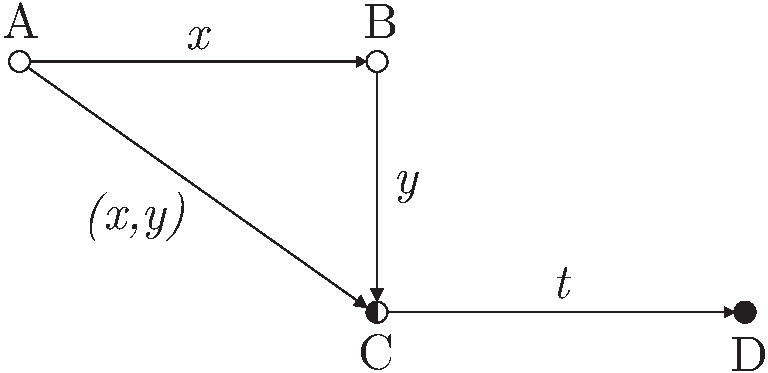
\includegraphics[width=0.7\textwidth]{files/methodeDerGeraden.pdf}
  \caption{Zwei verschiedene Möglichkeiten, zur semidiskreten Form C zu gelangen. Der Weg über B entspricht dabei der \emph{Methode der Geraden}. Im Punkt C verbleibt ein System gewöhnlicher DGLn, welches mit einem geeigneten Zeitschrittverfahren gelöst wird.}
  \label{fig:methodeDerGeraden}
\end{figure}

\subsection{DG/FV Hybridverfahren}
In natürlichen Einheiten kann die bezüglich $y$ diskretisierte LvNG allgemein durch
\begin{equation}
  {A}^y u_t(x,t) + {B}^y u_x(x,t) + {C}^y(x)u(x,t) = 0
  \label{eq:qschema}
\end{equation}
geschrieben werden. Die Matrizen  ${A}^y$, ${B}^y$ und ${C}^y$ resultieren in diesem Abschnitt aus einem FV Verfahren, können aber ebenso anderen Verfahren entstammen.

Dem FV Ansatz in \cite{lukas1} folgend wird das Intervall ${[-L_y/2,+L_y/2]}$ in $K_y$ Zellen unterteilt. Hieraus ergeben sich demnach $K+1$ \emph{interfaces} ${y_{\nicefrac{1}{2}}, y_{\nicefrac{3}{2}}, \dots, y_{K_y + \nicefrac{1}{2}} = -L_y/2, -L_y/2+\Delta y_1,\dots,+L_y/2}$.
Hierbei ist $\Delta y_i$ das Volumen der i-ten Zelle. Der Ansatz führt zu simplen Matrizen der Dimension ${K_y\times K_y}$ mit nicht verschwindenden Einträgen gemäß
\begin{equation}
  \begin{aligned}
  {A}^y_{i,i} &= \Delta y_i \\
  {B}^y_{i,i+1} &= -\frac{i}{2} \qquad
  {B}^y_{i+1, i} = +\frac{i}{2}  \\
  {C}^y_{i,i}(x) &= \mathrm{i} \frac{\Delta y_i}{4} (B(x, y_{i+\nicefrac{1}{2}}) + B(x, y_{i-\nicefrac{1}{2}}))  \\
  {C}^y_{i,i+1}(x) &= C^y_{i+1,i}(x) = \mathrm{i} \frac{\Delta y_i}{4} B(x, y_{i+\nicefrac{1}{2}})  \; .
  \end{aligned}
\end{equation}
Dieses Schema impliziert, dass $u(x,t)$ an den \emph{interfaces} als Mittelwert von rechts- und linksseitiger Zelle angenommen wird. Des weiteren sind  homogene Dirichlet Randbedingungen angenommen, also ${u(x,y_{\nicefrac{1}{2}}, t) = u(x,y_{K_y+\nicefrac{1}{2}}, t) = 0}$.

Die Matrix $B^y$ kann analytisch diagonalisiert werden. Es ist ${B^y = R\Lambda^y R^{\dagger}}$ mit der Diagonalmatrix
\begin{equation}
  \Lambda^y_{m,n} = \cos\left(\frac{2\pi n}{K_y+1}\right)\delta_{m,n}   \qquad m,n = 1,\dots,K_y
\end{equation}
und zugehörigen Eigenvektoren
\begin{equation}
  R_{m,n} = i^m \sin\left(\frac{mn\pi}{K_y +1} \right)   \qquad m,n = 1,\dots,K_y \; .
\end{equation}





% Die in Abbildung \ref{fig:pot1} eingezeichneten Längen werden wie in \cite{lukas1} zu
% \begin{align}
%   L_1 &= \SI{6}{\nano\meter}\\
%   L_2 &= \SI{5}{\nano\meter}\\
%   L_U &= \SI{30}{\nano\meter} \; .
% \end{align}
% gewählt. Hierin ist $L_U$ die Länge, über der die Spannung $U$ abfällt.

\todo{Idee: TF-Lösung für Überlagerung von l und r zeigen.}

% \section{Mathematische Aspekte der \lvn}
% Die eindimensionale Wellenfunktion $\Psi(x)$ eines Teilchens ist ein Vektor des unendlich-dimensionalen Hilbertraums $L^2(\mathbb{R})$ mit dem üblichen Skalarprodukt
% \begin{align}
%   \bra{\Psi}\ket{\Phi} = \int_{\mathbb{R}} \Psi^*(x)\Phi(x) \diff x \; .
% \end{align}
% Beschränken wir uns auf ein Rechengebiet $L$, so ist entsprechend $\Psi(x) \,\in\,L^2(L)$. Diskretisieren wir ferner das System, so wird der Hilbertraum endlichdimensional mit Dimension $N$. Dann ist die Dichtematrix in Gleichung \eqref{eq:lvn} eine Matrix der Form $\mathbb{C}^N \times \mathbb{C}^N$ und der Liouville-Operator ein "Superoperator" \cite{frensley2} der Form $(\mathbb{C}^N \times \mathbb{C}^N)\times(\mathbb{C}^N \times \mathbb{C}^N)$.
% Letztlich wird numerisch gesehen $N^2$ der Anzahl Freiheitsgrade entsprechen und die \lvn wird wieder eine Matrix-Vektor-Gleichung sein. Dazu wird $u(x,y)$ nicht als Matrix, sondern als Vektor der Länge $N^2$ geschrieben.
% \todo{Eigenschaften von B(x,y) und A. Hermitizität von $\mathcal{L}$ (frensley).}
